\section{Chimera Contacts protocol}
\label{app:chimeraContactsProtocol}%a012

Protocol designed to obtain contacts favorable and unfavorable (clashes or close contacts, where atoms are too close together) between any couple of chains of an atomic structure in \scipion by using \chimera. 

 \begin{itemize}
  \item Requirements to run this protocol and visualize results:
    \begin{itemize}
        \item \scipion plugin: \ttt{scipion-em-chimera}
    \end{itemize}
  \item \scipion menu:
   \ttt{Protocols SPA -> Model building} (\ffigure{fig:app_protocol_contacts_1} (A))
  
  \item Protocol form parameters (\ffigure{fig:app_protocol_contacts_1} (B)):
  
  \begin{figure}[H]
     \centering 
     \captionsetup{width=.7\linewidth} 
     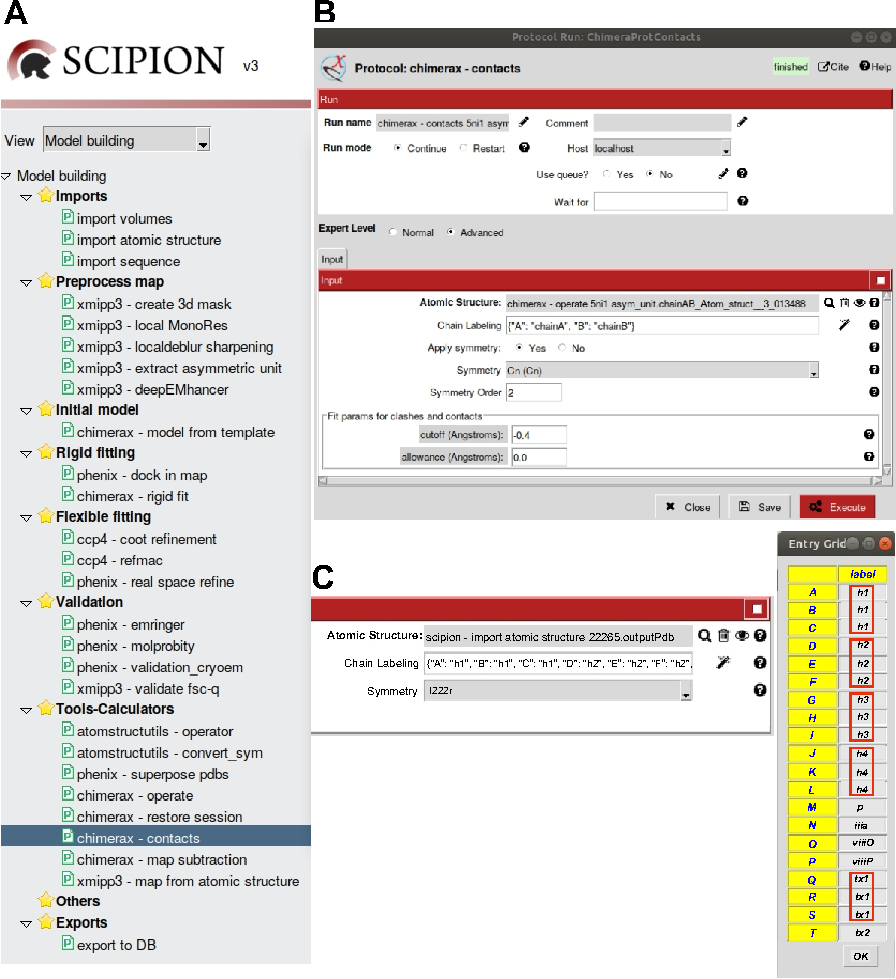
\includegraphics[width=0.90\textwidth]{Images_appendix/Fig155.pdf}
     \caption{Protocol \scommand{chimera contacts}. (A) Protocol location in \scipion menu. (B) Protocol form. (C) Protocol form detailing \ttt{Chain Labelling} for \ttt{I222r} symmetry.}
     \label{fig:app_protocol_contacts_1}
    \end{figure}

    \begin{itemize}
     \item \ttt{Atomic Structure}: Param to select one atomic structure previously downloaded or generated in \scipion with the aim of calculating contacts between any couple of chains.
     \item \ttt{Chain Labeling}: Param to asign a specific label for each one of the chains of the atomic structure. Chain labeling allows to group chains in order to get only contacts among chains from different groups. When two chains show the same label, contacts between any of these chains and an independent chain, or a chain that belongs to a different group, will be calculated. However, no contacts will be computed between chains included in the same group. \ffigure{fig:app_protocol_contacts_1} (C) shows an example of chain grouping in four different groups. Each one of these groups includes three chains: \ttt{$h1: [A, B, C]$; $h2: [D, E, F]$; $h3: [G, H, I]$; $h4: [J, K, L]$; $tx1: [Q, R, S]$}. The rest of chains remain as independent chains. There is a wizard on the right side of the \ttt{Chain Labeling} protocol form box to help the user to fill the form since it specifies the names of the different chains included in the \ttt{Atomic Structure} input. 
     \item \ttt{Apply symmetry}: Param that allows the user to select if symmetry has to be applied.
        \begin{itemize}
        \item Set to \ttt{Yes} if the \ttt{Atomic Structure} input is the unit cell of a macromolecule and you'd like to know the contacts between any two chains within the unit cell and the contacts between any chain of the unit cell and a chain from a neighbor unit cell. Consider, in this case, that only neigbor unit cells located at less than 3\AA\ of the input unit cell will be generated.\\
        WARNING: Be sure that the origin of coordinates equals the symmetry center of the input unit cell, in order to generate neighbor unit cells able to interact with the input unit cell.
        \item Set to \ttt{No} if you'd like to know the contacts between any two chains within the \ttt{Atomic Structure} input. 
        \end{itemize}
     \item \ttt{Symmetry}: If the user selects \ttt{Yes}, an additional protocol param box will interrogate about the type of symmetry. In order to reconstruct a macromolecule from a unit cell, symmetries allowed are cyclic (\ttt{Cn}), dihedral (\ttt{Dn}), tetrahedral (\ttt{T}), octahedral (\ttt{O}), and eight icosahedral symmetries (\ttt{I}). Each icosahedral symmetry shows its respective \chimera orientation (\url{https://www.cgl.ucsf.edu/chimera/current/docs/UsersGuide/midas/sym.html}):
            \begin{itemize}
            \item \ttt{I222}: \chimera orientation \ttt{222}; two-fold symmetry axes along the X, Y, and Z axes.
            \item \ttt{I222r}: \chimera orientation \ttt{222r}; idem except rotated 90\degree about Z. 
            \item \ttt{In25}: \chimera orientation \ttt{n25}; two-fold symmetry along Y and 5-fold along Z. 
            \item \ttt{In25r}: \chimera orientation \ttt{n25r}; idem except rotated 180\degree about X.
            \item \ttt{I2n3}: \chimera orientation \ttt{2n3}; two-fold symmetry along X and 3-fold along Z. 
            \item \ttt{I2n3r}: \chimera orientation \ttt{2n3r}; idem except rotated 180\degree about Y.
            \item \ttt{I2n5}: \chimera orientation \ttt{2n5}; two-fold symmetry along X and 5-fold along Z.
            \item \ttt{I2n5r}: \chimera orientation \ttt{2n5r}; idem  except rotated 180\degree about Y.
            \end{itemize}
    \item \ttt{Symmetry Order}: After selecting \ttt{Cn} or \ttt{Dn} symmetries, an additional protocol param box will interrogate about the symmetry order. An positive integer has to be written here. If the integer is \ttt{1} no symmetry will be applied. 
    \item \ttt{Tetrahedral orientation}: After selecting \ttt{T} symmetry, an additional protocol param box will interrogate about the tetrahedral orientation. The two \chimera orientation have been included (\url{https://www.cgl.ucsf.edu/chimera/current/docs/UsersGuide/midas/sym.html}):
            \begin{itemize}
            \item \ttt{222}: Two-fold symmetry axes along the X, Y, and Z axes, a three-fold along axis (1,1,1).
            \item \ttt{z3}: A three-fold symmetry axis along Z and another three-fold axis in the YZ plane.
            \end{itemize}
    \item \ttt{Fit params for clashes and contacts}: Advanced params that allow to modify interatomic distances in order to identify not only favorable interactions (by default), but also unfavorable ones (clashes) where atoms are too close together (\url{https://www.cgl.ucsf.edu/chimera/current/docs/UsersGuide/midas/sym.html}).
            \begin{itemize}
            \item \ttt{cutoff (Angstroms)}: Negative cutoff indicates favorable contacts; the default value to identify contacts is -0.4 (from 0.0 to -1.0). The default value to identify clashes is 0.6 (from 0.4 to 1.0). Large positive cutoff identifies the more severe clashes.
            \item \ttt{allowance (Angstroms)}: The default value to identify contacts is 0.0, whereas the default value to identify clashes is 0.4.
            \end{itemize}

    \end{itemize}

  \item Protocol execution:
  
  Adding specific protocol label is recommended in \ttt{Run name} section, at the form top. To add the label, open the protocol form, press the pencil symbol at the right side of \ttt{Run name} box, complete the label in the new opened window, press OK, and finally, close the protocol. This label will be shown in the output summary content (see below). If you want to run again this protocol, do not forget to set to \ttt{Restart} the \ttt{Run mode}.\\
  Press the \ttt{Execute} red button at the form bottom.
  
  \item Visualization of protocol results:
  After executing the protocol \scommand{chimera contacts} viewer window will be opened. This window includes three boxes (\ffigure{fig:contacts_results} (A)):
        \begin{itemize}
        \item \ttt{3D Visualization}: \chimera graphics window will be opened by selecting this option. The input atomic structure is shown, as well as the additional structure generated, if symmetry has been applied.
        \item \ttt{Interacting chains}: A text file will be opened detailing the number of atomic contacts, the models and the chains involved in contacts. Two scenarios have are examined:
            \begin{itemize}
            \item If \ttt{Apply symmetry} was set to \ttt{Yes}: If no chain groups have been established, all contacts between any couple of chains within the input atomic structure will be shown. Besides,``non-redundant'' contacts between any chain of the input unit cell structure and any chain of the neighbor unit cells will also be shown. By ``non-redundant'' contacts we define all those contacts that cannot be inferred by symmetry. An example of this type of contacts is shown in \ffigure{fig:schema_contacts} (A). In addition, input atomic structure is model \ttt{\#0}, whereas models generated by symmetry will be \ttt{\#1}, if only one is generated, and \ttt{\#1.1, \#1.2, \#1.3} and so on, if several models are generated. Each one of these models is supposed to be a neighbor unit cell located at less than 3 \AA\ from the input one.\\
            WARNING: If no additional models are generated at less than 3 \AA\ from the input one, consider the possibility that the symmetry center of the input structure does not coincide with the center of coordinates.
            \item If \ttt{Apply symmetry} was set to \ttt{No}: If no chain groups have been established, all contacts between any couple of chains within the input atomic structure will be shown (Example in \ffigure{fig:schema_contacts} (B)). There is only one model in this case, model \ttt{\#0}.
            \end{itemize}
        \item \ttt{Contacts between interacting chains}: This box allows to select a particular interaction between two chains to identify the residues involved in that interaction. The summary of results will be displayed in a text file. It includes the number of atom contacts between the residues of chain 1, model 1 and the residues of chain 2, model 2.
            \begin{itemize}
            \item \ttt{Swap chain columns in the summary of contacts}: Select \ttt{Yes} to display in the text file the number of contacts between the residues of chain 2, model 2 and the residues of chain 1, model 1. Otherwise, selecting \ttt{No}, the default order of columns will be shown.
            \item \ttt{Distance to group residues (Number of residues)}: Maximum number of residues between two residues that allows to group these two residues. Then, if two residues are closer than this number of residues (distance), they will be grouped. In a long list of grouped residues, the distance between two consecutive residues has to be lower than the set number of residues, 4 by default.  
            \item \ttt{Select two interacting chains and get the summary of contacts}: Select a particular interaction with the scroll arrow on the right and view the text file with the summary of contacts for that interaction.
            \end{itemize}
        \end{itemize}
   
  \item Summary content:
  
    \begin{itemize}
     \item Protocol output (below \scipion framework): No output information.
      
     \item \ttt{SUMMARY} box:\\No summary information.
    \end{itemize}
  
 \end{itemize}


